\documentclass[lettersize,journal]{IEEEtran}
\usepackage{flushend}
\usepackage{amsmath,amsfonts}
\usepackage{array}
\usepackage{textcomp}
\usepackage{tikz}
\usetikzlibrary{positioning}
\usetikzlibrary{math}
\usetikzlibrary{shapes}
\usepackage{pgfplots}
\usepackage{pgfplotstable}
\pgfplotsset{compat=1.7}
\usepgfplotslibrary{dateplot}
\setcounter{MaxMatrixCols}{20}
\usepackage{subfig}
\usepackage{stfloats}
\usepackage{url}
\usepackage{verbatim}
\usepackage{graphicx}
\usepackage{mathtools}
\hyphenation{op-tical net-works semi-conduc-tor IEEE-Xplore}
\def\BibTeX{{\rm B\kern-.05em{\sc i\kern-.025em b}\kern-.08em
    T\kern-.1667em\lower.7ex\hbox{E}\kern-.125emX}}
\usepackage{balance}
\usepackage[backend=bibtex, style=numeric, maxbibnames=10]{biblatex}
\bibliography{references}

% import custom function definitions
\usepackage{ifthen}
\pgfplotsset{
	SmallBarPlot/.style={font=\footnotesize, ybar, width=\linewidth, ymin=0, xmin=0, xmax=1.8, xtick=data, xticklabel style={text width=1.5cm, rotate=0, align=center}},
	SmallTimeSeriesPlot/.style={font=\footnotesize, width=\linewidth, height=2in, date coordinates in=x, xticklabel=\hour:\minute, ymin=0, ymax=100, legend pos=north west,
	major grid style={lightgray}, grid=both, minor grid style={lightgray!25}, minor tick num=1},
	SmallPointPlot/.style={font=\footnotesize, width=\linewidth, legend pos=south west, major grid style={lightgray},
	 grid=both, minor grid style={lightgray!25}, minor tick num=1}
	}


\newcommand\makeComparisonBarChartLog[4]{%
	\pgfplotstableread[col sep=comma]{#1}\table
	\begin{tikzpicture}
		\begin{axis}[SmallBarPlot, xticklabels from table={\table}{type}, ylabel=#2, ymode = log]
			\addplot [fill=blue!20, bar width=0.4] table [x expr=\coordindex*0.6 + 1 - 0.1, y=#3]{\table};
			\addplot [fill=red!20, bar width=0.4] table [x expr=\coordindex*0.6 + 1 + 0.1, y=#4]{\table};
		\end{axis}
	\end{tikzpicture} 
}

\newcommand\makeComparisonBarChartFour[6]{%
	\pgfplotstableread[col sep=comma]{#1}\table
	\begin{tikzpicture}
		\begin{axis}[SmallBarPlot, xticklabels from table={\table}{type}, ylabel=#2]
			\addplot [fill=blue!20, bar width=0.1] table [x expr=\coordindex*0.6 + 0.3, y=#3]{\table};
			\addlegendentry{#3}
			\addplot [fill=green!20, bar width=0.1] table [x expr=\coordindex*0.6 + 0.3, y=#4]{\table};
			\addlegendentry{#4}
			\addplot [fill=red!20, bar width=0.1] table [x expr=\coordindex*0.6 + 0.3, y=#5]{\table};
			\addlegendentry{#5} 
			\addplot [fill=purple!20, bar width=0.1] table [x expr=\coordindex*0.6 + 0.3, y=#6]{\table};
			\addlegendentry{#6}
			\legend{#3, #4, #5, #6}
		\end{axis}
	\end{tikzpicture} 
}
 
\newcommand\makeComparisonTotalPower[5]{%

\pgfplotstableread[col sep=comma]{#1}\firstTable
\pgfplotstableread[col sep=comma]{#2}\secondTable
\begin{tikzpicture}
	\begin{axis}[SmallTimeSeriesPlot, xlabel=Time (hr:min), ylabel=#3, ymax=1200, legend style={nodes={scale=0.7}}]
		\filldraw[fill=gray!40, opacity=0.3](625,0) rectangle (917,150);

		\addplot[blue, smooth] table [x = {time}, y = {facilitiesOut}]{\firstTable};
		\addplot[red, smooth] table [x = {time}, y = {facilitiesOut}]{\secondTable};

		\addplot[draw=green!20!black,fill=green!40!cyan!40, mark=pentagon*, only marks, mark size=3pt, y filter/.expression={y==0 ? nan:y}] table [x={time}, y={maxFacilitiesOut}]{\firstTable};
	        \addplot[draw=red,fill=green!10!orange!40, mark=pentagon*, only marks, mark size=3pt, y filter/.expression={y==0 ? nan:y}] table [x={time}, y={maxOnPeakOut}]{\firstTable};

		\addlegendimage{line width=10pt, color=gray!40, draw opacity=0.5}; 
	        \addplot[draw=green!20!black,fill=green!40!cyan!40, mark=pentagon*, only marks, mark size=3pt, y filter/.expression={y==0 ? nan:y}] table [x={time}, y={maxFacilitiesOut}]{\secondTable};
		\addplot[draw=red,fill=green!10!orange!40, mark=pentagon*, only marks, mark size=3pt, y filter/.expression={y==0 ? nan:y}] table [x={time}, y={maxOnPeakOut}]{\secondTable};   

	        \legend{#4, #5, Maximum Overall Average Power, Maximum On-Peak Average Power, On-Peak Time};
	\end{axis} 
\end{tikzpicture}

}

\newcommand\makeComparisonPower[5]{%
	\pgfplotstableread[col sep=comma]{#1}\firstTable
	\pgfplotstableread[col sep=comma]{#2}\secondTable
	\centering
	\begin{tikzpicture}
		\begin{axis}[SmallTimeSeriesPlot, ymin=-1, ymax=750, xlabel=Time (hr:min), ylabel=#3, legend style={nodes={scale=0.7}}]
			\addplot[blue, smooth] table [x = {time}, y = {meanBusPower}]{\firstTable};
			\addplot[red, smooth] table [x = {time}, y = {meanBusPower}]{\secondTable};
			\addplot[brown, smooth] table [x = {time}, y = {loadPower}]{\firstTable};
			\filldraw[fill=gray!40, opacity=0.3](625,0) rectangle (917,750);
			\addlegendimage{line width=10pt, color=gray!40, draw opacity=0.5}
			\legend{#4, #5, Uncontrolled Load, On-Peak Time}
		\end{axis} 
	\end{tikzpicture} 
}


%\bibliographystyle{ieeetr}
\begin{document}
\title{A Continuous Approach to Minimize Cost for Charging Electric Bus Fleets}
\author{Daniel Mortensen, Jacob Gunther, Greg Droge, Alexander Brown, Justin Whitaker\thanks{}}

\markboth{Transactions on Intelligent Transportation Systems}%
{}

\maketitle 
\begin{abstract}
	As transit authorities begin adopting Battery Electric Buses (BEBs), they must address the challenge of extended battery charging sessions while maintaining fixed bus schedules and managing the cost of energy.	This paper proposes a novel technique for minimizing the monthly cost of energy for operating electric bus fleets in the presence of time-varying uncontrolled loads.  The charging problem is cast as a constrained bin packing problem and expressed as a mixed integer linear program (MILP).  Among other things, we show that the proposed method significantly decreases demand on power infrastructure by temporally balancing the loads from buses with uncontrolled loads.  The bin packing formulation reduces the number of variables compared to prior discrete-time formulations, which reduces optimization runtime.
\end{abstract}

\begin{IEEEkeywords}
	Battery Electric Buses, Cost Minimization, Bin Packing, Mixed Integer Linear Program
\end{IEEEkeywords}

\section{Introduction}
\par  Battery powered electric motors for buses have long been a desired alternative to the internal combustion engine. The reduced maintenance \cite{poornesh_comparative_2020}, zero emissions \cite{kato_comparative_2013}, and access to renewable energy \cite{cheng_smart_2020} are but some of the benefits that have caused transit authorities to begin incorporating them into their bus fleets.  
\par Despite their benefits, transitioning to BEBs must address additional challenges, in particular, their extended refuel times. If a diesal or CNG bus runs low on fuel, refueling takes five to ten minutes.  An electric bus on the other hand may require several hours, causing the bus to fall behind schedule.
\par Maintaining a schedule while staying charged is one of the main challenges that BEBs face, and requires careful planning which must account for the battery discharge along routes, charge times, and a limited number of chargers. 
\par Charging while a bus is in motion, or dynamic charging, is one way to simplify a charge plan. There are a number of ways to do this including overhead \cite{csonka_optimization_2021} and inductive charging\cite{jeong_automatic_2018} \cite{balde_electric_2019}. An overhead charging scenario allows the bus to charge on overhead power lines while in motion while inductive charging relies on specialized hardware in the roads to inductively transfer energy when a bus passes overhead. Both methods remove the need to stop for service and allow an electrical vehicle to stay in service indefinately. They also require extensive infrastructure that may not be available.
\par In the absence of infrastructure, \cite{jain_battery_2020} and \cite{xian_zhang_optimal_2016} have proposed methods that exchange depleted batteries for fresh ones. Such a method would eliminate both the logistical challenges of planning and the infrastructure dependence of dynamic charging. The only drawback, is that BEBs are not built with battery exchanges in mind, therefore the task can require specialized hardware, technical expertise, or automation, all of which add complexity and cost.

\par One charge option that avoids both the infrastructural demands of dynamic charging and the technical difficulties of battery swapping is stationary charging, which plans rest periods into a bus's schedule during which that bus can charge \cite{whitaker_network_nodate}. Stationary charging is the least invasive form of bus charging because it only requires charging hardware at specific locations and makes no changes to bus batteries. There is extensive prior work in this area which, in addition to bus availability, has considered environmental impact \cite{zhou_bi-objective_2021}, battery health \cite{houbbadi_optimal_2019}, and the cost of electricity.
\par One drawback to using a stationary charging solution is that it does require significant rest periods for charging. One way to decrease the charge intervals is to use high power chargers, which deliver more energy in a smaller period of time. Large power demands however do increase the overall cost of energy because they must be supported by highly capable infrastructure \cite{stahleder_impact_2019}, \cite{deb_impact_2017}, \cite{boonraksa_impact_2019}. An effective charge plan must therefore balance the need to charge quickly with the desire to maintain a low power profile \cite{cheng_smart_2020}, \cite{ojer_development_2020}, \cite{qin_numerical_2016}, \cite{bagherinezhad_spatio-temporal_2020} which includes power used by BEBs and the power needed by other consumers.  
\par Because the additional power users are outside the control of the charge plan, their power requirements are referred to in this paper as "uncontrolled loads". Uncontrolled loads complicate the problem of finding an optimal charge plan. If a bus charges in the presence of a large uncontrolled load, the overall power profile is heightened, increasing cost for energy. 
\par A significant contribution of \cite{mortensen_comprehensive_2021} was how the authors minimized the the financial impact of charging in the presence of uncontrolled loads by formulating the charge problem as a graph and solving for the optimal path. The graph based approach represented time discretely, which lent itself well to integrating uncontrolled loads, which are sampled discretely in practice. 
\par Unfortunately, more temporal precision decreases the time step between sections in the graph, which leads to a larger graph and significantly increases the computational complexity. The authors of \cite{brown_position_nodate} compute the charge schedule continuously by formulating the charge problem as a bin packing problem \cite{Ma_Mixed-integer_2017}, yielding a precise time schedule for charging, but finding a continuous-time schedule that incorporates uncontrolled loads and minimizes a comprehensive cost function remains an open problem and is the focus of this paper. 
\par The rest of this paper is organized as follows: Section \ref{sec:4_formulation} discuses the basic problem formulation, Section \ref{sec:5_battery} discuses linear constraints that govern the behavior and limitations of the sate of charge. Section \ref{sec:uncontrolled} discuses how to incorporate uncontrolled loads into the optimization framework. Section \ref{sec:objective} explaines how the objective function is formed, and Section \ref{sec:results} discusses performance.

\section{Availability and Resource Contention\label{sec:4_formulation}}
The charge scheduling framework described in this paper is formulated as a constrained optimization problem that can be solved as a Mixed Integer Linear Program (MILP) of the form
\begin{equation}\label{eqn:MILP}\begin{matrix}
	\underset{\mathbf{y}}{\text{min}} \ \mathbf{y}^T\mathbf{g} \text{ subject to } \\
	\tilde{A}\mathbf{y} = \tilde{\mathbf{b}}, \ A\mathbf{y} \le \mathbf{b},
\end{matrix} \end{equation}
where $\mathbf{y}$, $\tilde{A}$, $A$, and $\mathbf{g}$ represent the solution vector, equality and inequality constraints, and cost vector respectively. In this paper, $\mathbf{y}$ is comprised of several variables, and is expressed as 
\begin{equation}\label{eqn:yDef}
	\mathbf{y} = \begin{bmatrix}
			\boldsymbol{\sigma} \\ 
			\mathbf{c}      \\ 
			\mathbf{s}      \\ 
			\mathbf{h}      \\ 
			\mathbf{k}      \\ 
			\mathbf{r}      \\ 
			\mathbf{g}      \\
			\mathbf{p}      \\ 
			q_{\text{on}}   \\ 
			q_{\text{all}}  \\
		     \end{bmatrix},
\end{equation}
where $\boldsymbol{\sigma}$, $\mathbf{c}$, $\mathbf{s}$, $\mathbf{h}$, $\mathbf{k}$, $\mathbf{r}$, $\mathbf{p}$, $q_{\text{on}}$, and $q_{\text{all}}$ will be developed through the course of this paper.
\par The cost function in \eqref{eqn:MILP} will be designed to model a realistic billing structure used by \cite{rocky_mountain_power_rocky_2021} and minimises the cost even in the presence of uncontrolled loads. Additionally, the constraints are designed to encorporate bus schedules, limit bus state of charges, and include a linear charge model calibrated on data from the Utah Transit Authority.
\subsection{Setup}
\par A solution to the bus charge problem includes both temporal and categorical information. The temporal aspect shows when and for how long a bus should charge and the categorical shows which bus must charge, indicating a solution with two dimensions.  The first dimension represents time continuously from left to right, and the second describes the buses as shown in Fig. \ref{fig:busTime1}.
\begin{figure*}
	\centering
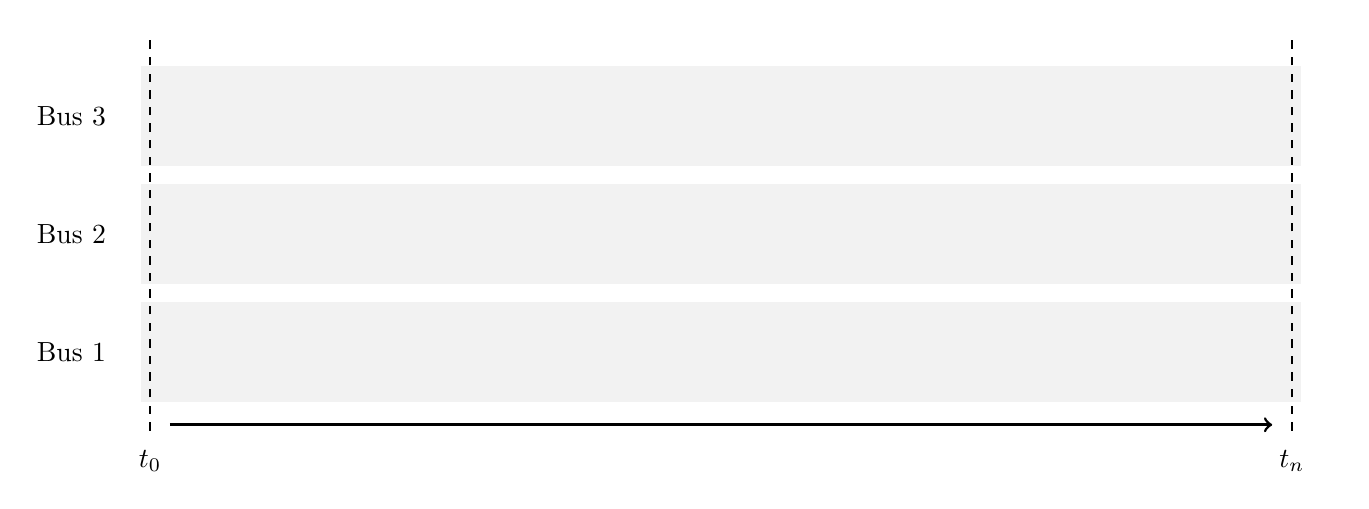
\begin{tikzpicture}
	\node[rectangle, fill=gray!10, minimum width=5.8in, minimum height=0.5in](bus1Box) at (7.75,1){};
	\node(bus1BoxLabel) at (-0.5, 1){Bus 1}; 

	\node[rectangle, fill=gray!10, minimum width=5.8in, minimum height=0.5in](bus2Box) at (7.75,2.5){};
	\node(bus1BoxLabel) at (-0.5, 2.5){Bus 2};

	\node[rectangle, fill=gray!10, minimum width=5.8in, minimum height=0.5in](bus3Box) at (7.75,4){};
	\node(bus1BoxLabel) at (-0.5, 4){Bus 3};

	\node[label=below:$t_0$](origin) at (0.5,0){};
	\node(yAxes) at (15.5,0){};
	\node(xAxes) at (0.5,5){};
	\node[label=below:$t_n$](bottomRight) at (15,0){};
	\node(topRight) at (15,5){};
	\draw[dashed, line width=0.5pt] (origin.center) -- (xAxes.center); 
	\draw[dashed, line width=0.5pt] (bottomRight.center) -- (topRight.center);
	\node(t0) at (0.75,-0.05){};
	\node(tn) at (14.75,-0.05){};
	\draw[->, line width=1pt] (t0.north) -- (tn.north); 
\end{tikzpicture}
	\caption{Description of the bus and time axis}
	\label{fig:busTime1}
\end{figure*}

\par Each bus follows a schedule of arrival and departure times, where the $i^{\text{th}}$ bus's $j^{\text{th}}$ stop begins at arrival time $a_{ij}$ and terminates at departure time $d_{ij}$ (see Fig. \ref{fig:busTime3}).  A bus can be assigned to charge anytime the bus is in the station such that the charge start time, $c_{ij}$, is greater than or equal to $a_{ij}$, and the charge stop time, $s_{ij}$, is less than the departure time $d_{ij}$ as shown in Fig. \ref{fig:busTime3}. In the context of a MILP, the arrival and departure times $a_{ij}$ and $d_{ij}$ are known ahead of time and charge times $c_{ij}$ and $s_{ij}$ are optimization variables. 
\begin{figure*}
\centering
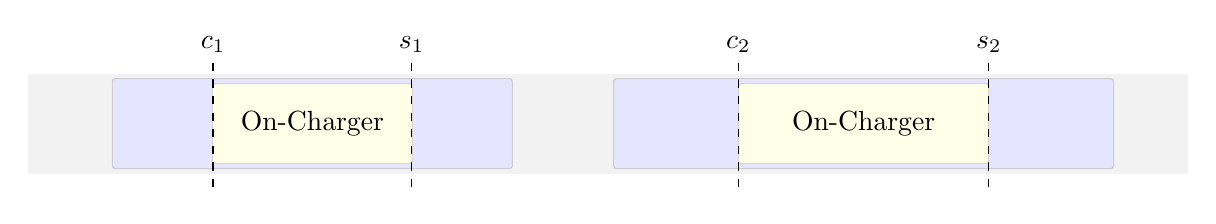
\begin{tikzpicture} 
	\node[rectangle, fill=gray!10, minimum width=5.8in, minimum height=0.5in](busSched) at (7.75,1){}; 

	\node[rectangle, draw=blue!10!black!20, fill=blue!10, minimum width=2in, minimum height=0.45in, rounded corners=1pt](busAvail1) at (4,1){In-Station};
	\node[rectangle, draw=blue!10!black!20, fill=blue!10, minimum width=2.5in, minimum height=0.45in, rounded corners=1pt](busAvail2) at (11,1){In-Station};

	\node[rectangle, draw=yellow!10!black!20, fill=yellow!10, minimum width=1in, minimum height=0.4in, rounded corners=1pt](busAvail1) at (4,1){On-Charger};
	\node[rectangle, draw=yellow!10!black!20, fill=yellow!10, minimum width=1.25in, minimum height=0.4in, rounded corners=1pt](busAvail2) at (11,1){On-Charger};


	\node(firstATop) at (2.74,2){$c_1$};
	\node(firstABtm) at (2.74,0.2){};
	\draw[dashed, line width=0.5pt](firstATop) -- (firstABtm.center);
	\node(firstDTop) at (5.26,2){$s_1$};
	\node(firstDBtm) at (5.26,0.2){};
	\draw[dashed, line width=0.5pt](firstDTop) -- (firstDBtm.center);

	\node(secondATop) at (9.41,2){$c_2$};
	\node(secondABtm) at (9.41,0.2){};
	\draw[dashed, line width=0.5pt](secondATop) -- (secondABtm.center);
	\node(secondDTop) at (12.59,2){$s_2$};
	\node(secondDBtm) at (12.59,0.2){};
	\draw[dashed, line width=0.5pt](secondDTop) -- (secondDBtm.center);


\end{tikzpicture}
\caption{Bus Charging}
\label{fig:busTime3}
\end{figure*}

\subsection{Constraints}
The relationship between the arrival, departure, and charge intervals for the $i^{\text{th}}$ bus at the $j^{\text{th}}$ stop can be expressed as a set of inequality constraints such that
\begin{equation}\begin{aligned}
	a_{ij} &< c_{ij} \\
	c_{ij} &< s_{ij} \\
	s_{ij} &< d_{ij}.
\end{aligned}\end{equation}
These constraints can be rewritten such that the optimization variables are on the left, the known parameters are on the right, and the relationship is "less than" (or standard form) such that
\begin{equation}\begin{aligned}
	-c_{ij} &< -a_{ij}\\
	c_{ij} - s_{ij} &< 0\\
	s_{ij} &< d_{ij}.
\end{aligned}\end{equation}
Standard form is preferred because it provides a standard way to represent equations. Having the optimization variables on the left also allows the expression to be written using matrix notation as 
\begin{equation}\label{eqn:timeConstraint}
	\begin{bmatrix} -1 & 0 \\
	                 1 & -1 \\
		0 & 1\end{bmatrix} \begin{bmatrix} c_{ij} \\ s_{ij}\end{bmatrix} \le \begin{bmatrix}-a_{ij} \\ 0 \\ d_{ij} \end{bmatrix}.
\end{equation}
	However, because all constraints must follow the form $A\mathbf{y} = \mathbf{b}$ as shown in \eqref{eqn:MILP}, \eqref{eqn:timeConstraint} is expressed in terms of $\mathbf{y}$ such that
\begin{equation} \begin{aligned}
	\begin{bmatrix}
		-1^c_{ij} & 0 & \hdots &  0        \\
	         1^c_{ij} & 0 & \hdots & -1^d_{ij} \\
		 0        & 0 & \hdots &  1^d_{ij} \\ 
	\end{bmatrix}
	\mathbf{y} &\le 
	\begin{bmatrix}
	        -a_{ij} \\ 
		 0      \\ 
		 d_{ij} \\
	\end{bmatrix} \ \forall i,j \\
	A_1\mathbf{y} &\le \mathbf{b}_1,
\end{aligned} \end{equation}
	where $1^c_{ij}$ is $1$ at the location corresponding to $c_{ij}$, $1^d_{ij}$ is $1$ at the location corresponding to $d_{ij}$, and $A_1$ and $\mathbf{b}_1$ stack the constraints given in \eqref{eqn:timeConstraint} for all $i,j$.
	\par The decision variables $s_{ij}$ and $c_{ij}$ from \eqref{eqn:timeConstraint} show when a bus must start and finish charging, but do not indicate on which charger. The variable $\boldsymbol{\sigma}$ from \eqref{eqn:yDef} is a vector of binary variables. Each element of $\boldsymbol{\sigma}$ is denoted $\sigma_{ijk}$ and is $1$ when bus $i$ charges during the $j^{\text{th}}$ stop at charger $k$. Because a bus can only charge at one charger at a time, the values in $\boldsymbol{\sigma}$ must be constrained such that
\begin{equation}
	\begin{aligned}
		\sum_k \sigma_{ijk} \le 1 \ \forall i,j
	\end{aligned}
\end{equation} 
or in standard form as 
\begin{equation} \begin{aligned}
	\begin{bmatrix}1_{ij1} & 0 & \hdots & 0 & 1_{ijk} \end{bmatrix} \mathbf{y} &\le \mathbf{1} \ \forall i,j\\
		A_2\mathbf{y} & \le \mathbf{b}_2,
\end{aligned} \end{equation}
where $1_{ijk}$ represents a $1$ at the location corresponding to $\sigma_{ijk}$.
	The variable $\sigma_{ijk}$ is used in several scenarios. The first is to ensure that buses without charge assignments have a charge time of zero by constraining $s_{ij}$ and $c_{ij}$ to be the same value. This is done by letting
	\begin{equation}\label{eqn:A3}\begin{aligned}
	s_{ij} - c_{ij} &\le M\sum_{k}\sigma_{ijk} \\
	s_{ij} - c_{ij} - \sum_{k}\sigma_{ijk}M &\le 0\\
	\begin{bmatrix} 1_s & -1_c & -M_{\sigma} \end{bmatrix}\begin{bmatrix}s_{ij} \\ c_{ij} \\ \sigma_{ij1} \\ \vdots \\ \sigma_{ijk} \end{bmatrix} &\le 0 \ \forall i,j 
\end{aligned} \end{equation}
	where $M$ is the maximum difference between $s_{ij}$ and $c_{ij}$, or the number of seconds in a day, denoted $\text{nTime}$ and $M_\sigma$ represents multiple values of $M$ at locations corresponding to each $\sigma_{ijk}$. The constraints in \eqref{eqn:A3} can be appropriately zero padded and stacked for all $i,j$ to form the linear expression
	\begin{equation} 
		A_3\mathbf{y} \le \mathbf{b}_3
	\end{equation}
	\par The values in $\boldsymbol{\sigma}$, $\mathbf{c}$, and $\mathbf{s}$ form a complete charge plan representation were $c_{ij}$ and $s_{ij}$ describe time periods when a bus will charge and $\sigma_{ijk}$ gives which charger to use. (see Fig. \ref{fig:busTime4}).
\begin{figure*}
	\centering
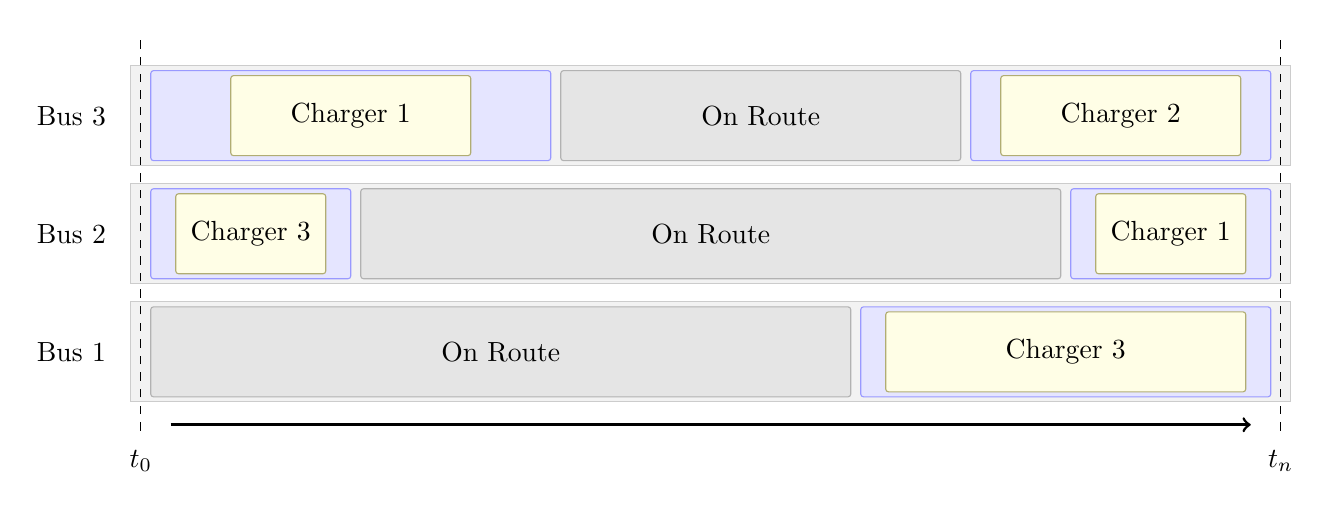
\begin{tikzpicture}
	\node[rectangle, draw=gray!40, fill=gray!10, minimum width=5.8in, minimum height=0.5in](charger1Box) at (3in,1){};
	\node(bus1BoxLabel) at (-0.5, 1){Bus 1}; 

	\node[rectangle, draw=gray!40, fill=gray!10, minimum width=5.8in, minimum height=0.5in](charger2Box) at (3in,2.5){};
	\node(bus1BoxLabel) at (-0.5, 2.5){Bus 2};

	\node[rectangle, draw=gray!40, fill=gray!10, minimum width=5.8in, minimum height=0.5in](charger3Box) at (3in,4){};
	\node(bus1BoxLabel) at (-0.5, 4){Bus 3};

	\node[label=below:$t_0$](origin) at (0.15in,0){};
	\node(xAxes) at (0.15in,5){};
	\node[label=below:$t_n$](bottomRight) at (5.85in,0){};
	\node(topRight) at (5.85in,5){};
	\draw[dashed, line width=0.5pt] (origin.center) -- (xAxes.center); 
	\draw[dashed, line width=0.5pt] (bottomRight.center) -- (topRight.center);
	\node(t0) at (0.3in,-0.05){};
	\node(tn) at (5.7in,-0.05){};
	\draw[->, line width=1pt] (t0.north) -- (tn.north); 

	% draw bus 3 boxes
	\node[rectangle, draw=blue!40, fill=blue!10, minimum width=2in, minimum height=0.45in, rounded corners=1pt](bus1Avail1) at (1.2in,4){};
	\node[rectangle, draw=yellow!50!black!70, fill=yellow!10, minimum width=1.2in, minimum height=0.4in, rounded corners=1pt](bus1Time1) at (1.2in,4){Charger 1};

	\node[rectangle, draw=black!30, fill=black!10, minimum width=2in, minimum height=0.45in, rounded corners=1pt](bus2Time1) at (3.25in,4){On Route};

	\node[rectangle, draw=blue!40, fill=blue!10, minimum width=1.5in, minimum height=0.45in, rounded corners=1pt](bus1Avail1) at (5.05in,4){};
	\node[rectangle, draw=yellow!50!black!70, fill=yellow!10, minimum width=1.2in, minimum height=0.40in, rounded corners=1pt](bus3Time1) at (5.05in,4){Charger 2};

	% draw bus 2 boxes
	\node[rectangle, draw=blue!40, fill=blue!10, minimum width=1in, minimum height=0.45in, rounded corners=1pt](bus1Avail1) at (0.7in,2.5){};
	\node[rectangle, draw=yellow!50!black!70, fill=yellow!10, minimum width=0.75in, minimum height=0.4in, rounded corners=1pt](free1) at (0.7in,2.5){Charger 3};

	\node[rectangle, draw=black!30, fill=black!10, minimum width=3.5in, minimum height=0.45in, rounded corners=1pt](bus3Time2) at (3.0in,2.5){On Route};

	\node[rectangle, draw=blue!40, fill=blue!10, minimum width=1.0in, minimum height=0.45in, rounded corners=1pt](bus1Avail1) at (5.3in,2.5){};
	\node[rectangle, draw=yellow!50!black!70, fill=yellow!10, minimum width=0.75in, minimum height=0.4in, rounded corners=1pt](free2) at (5.3in,2.5){Charger 1};

	% draw bus 1 boxes 
	\node[rectangle, draw=black!30!, fill=black!10, minimum width=3.5in, minimum height=0.45in, rounded corners=1pt](bus3Time2) at (1.95in,1){On Route}; 

	\node[rectangle, draw=blue!40, fill=blue!10, minimum width=2.05in, minimum height=0.45in, rounded corners=1pt](bus1Avail1) at (4.775in,1){};
	\node[rectangle, draw=yellow!50!black!70, fill=yellow!10, minimum width=1.8in, minimum height=0.4in, rounded corners=1pt](bus1Time2) at (4.775in,1){Charger 3};
\end{tikzpicture}
	\caption{Reserving time slots on chargers}
	\label{fig:busTime4}
\end{figure*}

	The variable $\sigma_{ijk}$ is also necessary to eliminate situations where more then one bus is assigned to a charger at the same time. Note that this can only happen when $a_{ij}$ for bus $i$ is less than $d_{i^{'}j^{'}}$ for bus $i^{'}$ as shown in Fig. \ref{fig:potentialOverlap}. Let $\mathcal{S}$ be the set of all bus break pairs such that $\left (ij, \ i^{`}j^{`} \right ) \in \mathcal{S}$ if overlap is possible between bus $i$ and bus $i^{`}$ during the $j$ and $j^{`}$ stops respectively. Charging overlap can be avoided by constraining
\begin{figure}[ht!]
	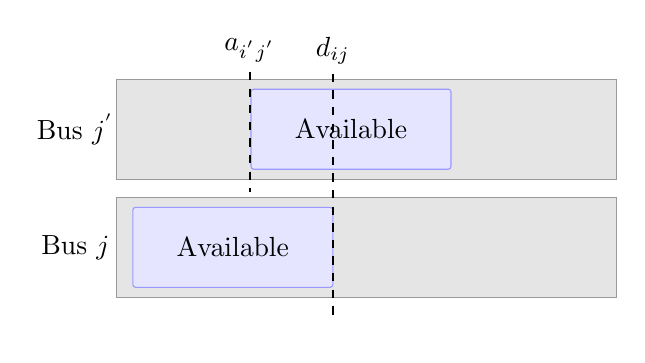
\begin{tikzpicture} 
		\node[rectangle, draw=black!40, fill=black!10, minimum width=2.5in, minimum height=0.5in](charger1Box) at (3.2,1){};
		\node(bus1BoxLabel) at (-0.5, 1){Bus $j$}; 
		\node[rectangle, draw=black!40, fill=black!10, minimum width=2.5in, minimum height=0.5in](charger2Box) at (3.2,2.5){};
		\node(bus1BoxLabel) at (-0.5, 2.5){Bus $j^{'}$};
		\node[rectangle, draw=blue!40, fill=blue!10, minimum width=1in, minimum height=0.4in, rounded corners=1pt] at (1.5,1){Available};
		\node[rectangle, draw=blue!40, fill=blue!10, minimum width=1in, minimum height=0.4in, rounded corners=1pt] at (3,2.5){Available};
		\node(aJPrimeHigh) at (1.72,3.5){$a_{i^{'}j^{'}}$};
		\node(aJPrimeLow) at (1.72,1.7){};
		\node(dJHigh) at (2.77,3.5){$d_{ij}$};
		\node(dJLow) at (2.77,0.0){};
		\draw[dashed, line width=0.5pt] (aJPrimeHigh) -- (aJPrimeLow.center);
		\draw[dashed, line width=0.5pt] (dJHigh) -- (dJLow);
	\end{tikzpicture}
	\caption{Potential Overlap}
	\label{fig:potentialOverlap}
\end{figure}



\begin{equation}\label{eqn:overlapConstraints1}
	\begin{array}{c}
		c_{i^{`}j^{`}} > s_{ij} \\
		\text{or} \\
		c_{ij} > s_{i^{`}j^{`}} 
	\end{array} \ \forall \left ( ij, \ i^{`}j^{`}\right ) \in \mathcal{S}
\end{equation}
	Let $l_{\left( ij, \ i^{`}j^{`}\right )}$ be a binary decision variable that is $1$ when $c_{i^{'}j^{'}} > s_{ij}$, and $0$ when $c_{ij} > s_{i^{'}j^{'}}$. The expression from \eqref{eqn:overlapConstraints1} can be rewritten as
	\begin{equation} \label{eqn:overlapConstraints2}\begin{aligned}
	c_{i^{`}j^{`}} - s_{ij}  &> -Ml_{\left( ij, \ i^{`}j^{`}\right )} \\
	c_{ij}-s_{i^{`}j^{`}} &>  -M(1 - l_{\left( ij, \ i^{`}j^{`}\right )}) \\
\end{aligned}\end{equation}
	However, this constraint is only necessary when buses $i$ and $i^{`}$ must use the same charger. This can be remedied as
\begin{equation}\label{eqn:overlapConstraints3}\begin{aligned}
	c_{i^{'}j^{'}} - s_{ij} &> M\left[(\sigma_{i^{'}j^{'}k} + \sigma_{ijk}) - 2\right] - Ml_{\left( ij, \ i^{`}j^{`}\right )} \ \forall k \\
	c_{ij} - s_{i^{'}j^{'}} &> M\left[(\sigma_{i^{'}j^{'}k} + \sigma_{ijk}) - 2\right] - M(1 - l_{\left( ij, \ i^{`}j^{`}\right )})\ \forall k \\
\end{aligned}\end{equation}
When $(\sigma_{i^{'}j^{'}k} + \sigma_{ijk}) < 2$, \eqref{eqn:overlapConstraints3} is trivially satisfied for all values of $c_{i^{'}j^{'}}$ and $s_{ij}$. When $\sigma_{i^{'}j^{'}k} = \sigma_{ijk} = 1$, \eqref{eqn:overlapConstraints3} simplifies to \eqref{eqn:overlapConstraints2}. Equation \eqref{eqn:overlapConstraints3} can be expressed in standard form as 
	\begin{equation}\label{eqn:overlapConstraints3}\begin{aligned}
		-c_{i^{`}j^{`}} + s_{ij} + M\sigma_{i^{'}j^{'}k} + M\sigma_{ijk} - Ml_{iji^{`}j^{`}}&\le 2M  \ \forall k\\
		-c_{ij} + s_{i^{`}j^{`}} + M\sigma_{i^{'}j^{'}k} + M\sigma_{ijk} + Ml_{iji^{`}j^{`}}&\le 3M  \ \forall k\\
	\end{aligned}\end{equation}
	and finally as
	\begin{equation}\begin{aligned} 
		\begin{bmatrix} 
			-1 & 0 &  0 & 1 & M & M & -M \\
			 0 & 1 & -1 & 0 & M & M &  M \\
		\end{bmatrix} 
		\begin{bmatrix}
			c_{i^{'}j^{'}}       \\ 
			s_{i^{'}j^{'}}       \\
			c_{ij}               \\
			s_{ij}               \\ 
			\sigma_{i^{'}j^{'}k} \\ 
			\sigma_{ijk}         \\
			l_{iji^{`}j^{`}}     \\
		\end{bmatrix} &\le 
		\begin{bmatrix} 
			2M \\ 
			3M \\
		\end{bmatrix} \forall k
	\end{aligned} \end{equation}
	The constraints in \eqref{eqn:overlapConstraints3} can be repeated for all $\left ( ij, \ i^{`}j^{`} \right ) \in \mathcal{S}$ and concatenated into a single matrix expression
	\begin{equation}\begin{aligned} 
		A_4\mathbf{y} & \le \mathbf{b}_4 \\
	\end{aligned} \end{equation} 

\section{Battery State of Charge}
BEBs must also maintain their state of charge above a minimum threshold, denoted $h_{\text{min}}$. Let $h_{ij+1}$ be the state of charge for bus $i$ at the beginning of stop $j$. Each bus has an initial state of charge defined by $h_{i0}$ as shown in figure \ref{fig:hPlacement}. 
\begin{figure*}
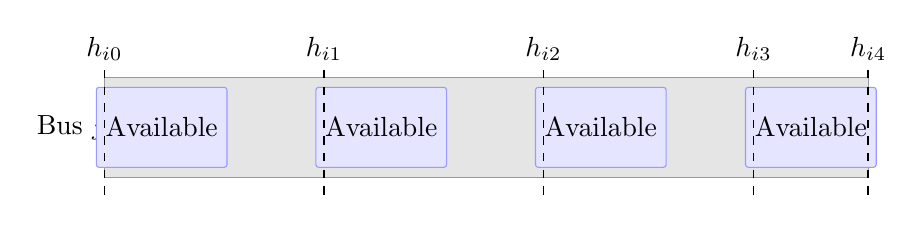
\begin{tikzpicture}
\node[rectangle, draw=black!40, fill=black!10, minimum width=0.8\textwidth, minimum height=0.5in](charger1Box) at (0.5\textwidth,1){};
	\node(bus1BoxLabel) at (0.065\textwidth, 1){Bus $j$}; 
	\node[rectangle, draw=blue!40, fill=blue!10, minimum width=0.12\textwidth, minimum height=0.4in, rounded corners=1pt] at (0.16\textwidth,1){Available};
	\node[rectangle, draw=blue!40, fill=blue!10, minimum width=0.12\textwidth, minimum height=0.4in, rounded corners=1pt] at (0.39\textwidth,1){Available};
	\node[rectangle, draw=blue!40, fill=blue!10, minimum width=0.12\textwidth, minimum height=0.4in, rounded corners=1pt] at (0.62\textwidth,1){Available};
	\node[rectangle, draw=blue!40, fill=blue!10, minimum width=0.12\textwidth, minimum height=0.4in, rounded corners=1pt] at (0.84\textwidth,1){Available};

	\node(h0High) at (0.1\textwidth,2){$h_{i0}$};
	\node(h0Low) at (0.1\textwidth,0.05){};
	\draw[dashed, line width=0.5pt] (h0High) -- (h0Low.center);

	\node(h1High) at (0.33\textwidth,2){$h_{i1}$};
	\node(h1Low) at (0.33\textwidth,0.05){};
	\draw[dashed, line width=0.5pt] (h1High) -- (h1Low.center);

	\node(h0High) at (0.56\textwidth,2){$h_{i2}$};
	\node(h0Low) at (0.56\textwidth,0.05){};
	\draw[dashed, line width=0.5pt] (h0High) -- (h0Low.center);

	\node(h0High) at (0.78\textwidth,2){$h_{i3}$};
	\node(h0Low) at (0.78\textwidth,0.05){};
	\draw[dashed, line width=0.5pt] (h0High) -- (h0Low.center);

	\node(h0High) at (0.9\textwidth,2){$h_{i4}$};
	\node(h0Low) at (0.9\textwidth,0.05){};
	\draw[dashed, line width=0.5pt] (h0High) -- (h0Low.center);
\end{tikzpicture}
\caption{State of Charge Variables}
\label{fig:hPlacement}
\end{figure*}

This can be constrained as
\begin{equation}\label{eqn:initialSoc0}
	h_{i0} = \eta_{i} \ \forall i.
\end{equation}
where $\eta_{i}$ is the initial state of charge for bus $i$.
Equation \ref{eqn:initialSoc0} can be expressed in standard form such that
\begin{equation} \begin{aligned}
	\begin{bmatrix}0 & 0 & \hdots & 0 & 1_i& 0 \end{bmatrix}\mathbf{y} &= \eta_i \ \forall i \\
		\tilde{A}_1\mathbf{y} &= \tilde{\mathbf{b}}_1
\end{aligned} \end{equation}
\begin{figure*}
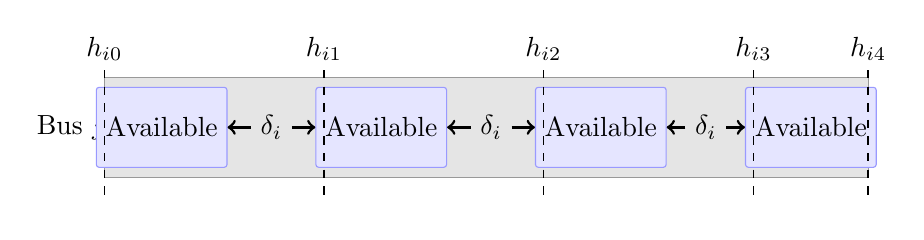
\begin{tikzpicture}
\node[rectangle, draw=black!40, fill=black!10, minimum width=0.8\textwidth, minimum height=0.5in](charger1Box) at (0.5\textwidth,1){};
	\node(bus1BoxLabel) at (0.065\textwidth, 1){Bus $j$}; 
	\node[rectangle, draw=blue!40, fill=blue!10, minimum width=0.12\textwidth, minimum height=0.4in, rounded corners=1pt](avail1) at (0.16\textwidth,1){Available};
	\node[rectangle, draw=blue!40, fill=blue!10, minimum width=0.12\textwidth, minimum height=0.4in, rounded corners=1pt](avail2) at (0.39\textwidth,1){Available};
	\node[rectangle, draw=blue!40, fill=blue!10, minimum width=0.12\textwidth, minimum height=0.4in, rounded corners=1pt](avail3) at (0.62\textwidth,1){Available};
	\node[rectangle, draw=blue!40, fill=blue!10, minimum width=0.12\textwidth, minimum height=0.4in, rounded corners=1pt](avail4) at (0.84\textwidth,1){Available};

	\node(h0High) at (0.1\textwidth,2){$h_{i0}$};
	\node(h0Low) at (0.1\textwidth,0.05){};
	\draw[dashed, line width=0.5pt] (h0High) -- (h0Low.center);

	\node(h1High) at (0.33\textwidth,2){$h_{i1}$};
	\node(h1Low) at (0.33\textwidth,0.05){};
	\draw[dashed, line width=0.5pt] (h1High) -- (h1Low.center);

	\node(h0High) at (0.56\textwidth,2){$h_{i2}$};
	\node(h0Low) at (0.56\textwidth,0.05){};
	\draw[dashed, line width=0.5pt] (h0High) -- (h0Low.center);

	\node(h0High) at (0.78\textwidth,2){$h_{i3}$};
	\node(h0Low) at (0.78\textwidth,0.05){};
	\draw[dashed, line width=0.5pt] (h0High) -- (h0Low.center);

	\node(h0High) at (0.9\textwidth,2){$h_{i4}$};
	\node(h0Low) at (0.9\textwidth,0.05){};
	\draw[dashed, line width=0.5pt] (h0High) -- (h0Low.center);

	\node(delta1) at (0.275\textwidth,1){$\delta_i$};
	\draw[->, line width=1pt] (delta1.west) -- (avail1.east);
	\draw[->, line width=1pt] (delta1.east) -- (avail2.west);
	\node(delta2) at (0.505\textwidth,1){$\delta_i$}; 
	\draw[->, line width=1pt] (delta2.west) -- (avail2.east);
	\draw[->, line width=1pt] (delta2.east) -- (avail3.west);
	\node(delta3) at (0.73\textwidth,1){$\delta_i$}; 
	\draw[->, line width=1pt] (delta3.west) -- (avail3.east);
	\draw[->, line width=1pt] (delta3.east) -- (avail4.west);
\end{tikzpicture}
\caption{Placement for $\delta_i$}
\label{fig:hPlacement}
\end{figure*}

\par The transition from $h_{ij}$ to $h_{ij+1}$ is computed as the sum of battery effects due to charging and discharging. The discharge from operating bus $i$ over one route loop is denoted $\delta_i$. The increase in battery state of charge follows a linear charge model such that the increase is equal to the energy rate, denoted $p$, times the time spent charging, denoted $\Delta_{\text{sc}}$.
The total change from $h_{ij}$ to $h_{ij+1}$ can be expressed as
\begin{equation}
	h_{ij+1} = h_{ij} + \Delta T\cdot p - \delta_i.
\end{equation}
The value for $\Delta T$ can also be expressed in terms of the difference between $a_{ij}$ and $d_{ij}$ such that
\begin{equation}
	h_{ij+1} = h_{ij} + p\cdot \left ( s_{ij} - c_{ij} \right ) - \delta_i.
\end{equation}
This is only the case, however, if the bus is assigned to a charger at stop $j$, otherwise the net increase is zero. This piecewise behavior can be modeled by using the charger selection variables, $\sigma_{ijk}$ such that
\begin{equation}\label{eqn:bilinear}
	h_{ij+1} = h_{ij} - \delta_i + p\cdot\left(\sum_k\sigma_{ijk}\right )\cdot(s_{ij} - c_{ij}) 
\end{equation}
but because equation \ref{eqn:bilinear} introduces a bilinear term, the behavior or $h$ is alternatively expressed as
\begin{equation} \begin{aligned}
	h_{ij+1} & \le h_{ij} - \delta_i + p\cdot(s_{ij} - c_{ij}) - M(1 - \sum_k\sigma_{ijk})\\
	h_{ij+1} & \ge h_{ij} - \delta_i + p\cdot(s_{ij} - c_{ij}) + M(1 - \sum_k\sigma_{ijk})\\
	h_{ij+1} & \le h_{ij} - \delta_i - M\sum_k\sigma_{ijk}\\
	h_{ij+1} & \ge h_{ij} - \delta_i + M\sum_k\sigma_{ijk}\\
\end{aligned} \end{equation}
Which can be expressed in standard form as
\begin{equation} \begin{aligned}
	 h_{ij+1} - h_{ij} - p\cdot s_{ij} + p\cdot c_{ij} - M\sum_k\sigma_{ijk} &\le -\left(\delta_i + M\right) \\
	-h_{ij+1} + h_{ij} + p\cdot s_{ij} - p\cdot c_{ij} - M\sum_k\sigma_{ijk} &\le \delta_i - M \\
	 h_{ij+1} - h_{ij} + M\sum_k\sigma_{ijk} &\le -\delta_i \\
	-h_{ij+1} + h_{ij} + M\sum_k\sigma_{ijk} & \le \delta_i \\
\end{aligned} \end{equation}
and finally,
\begin{equation} \label{eqn:socDynamic1} \begin{aligned}
	\begin{bmatrix}1  & -1 & -p & p   & -M_k \\
		       -1 & 1  & p  & -p  & -M_k \\
		       1  & -1 & 0             & 0              & M_k  \\
		       -1 & 1  & 0             & 0              & M_k  \\
	\end{bmatrix}
	\begin{bmatrix}h_{ij+1} \\ h_{ij} \\ s_{ij} \\ c_{ij} \\ \sigma_{ijk} \end{bmatrix} &\le 
		\begin{bmatrix}-\delta_i - M \\ \delta_i - M \\ -\delta_i \\ \delta_i \end{bmatrix} \ \forall i,j \\
			A_{ij}\mathbf{y} &\le \mathbf{b}_{ij} \ \forall i,j
\end{aligned} \end{equation}
If the bus ends the day in the station (as is common), there is one final $h$ value that is computed without a route discharge parameter. Let $\mathcal{S}$ be the set of all $i,j$ where $h_{ij+1}$ describes the final state of charge value for bus $i$. Equation \ref{eqn:socDynamic1} can be reexpressed as 
\begin{equation}\label{eqn:socDynamic2} 
	\mathbf{b}_{ij} = 
	\begin{dcases}
		% first case
		\begin{bmatrix} -\delta_i - M \\
			         \delta_i - M \\
		                -\delta_i     \\
		                 \delta_i 
		\end{bmatrix} & \forall i,j \ni h_{ij+1} \notin \mathcal{S} \\
		% second case
		\omit \hfil$\begin{bmatrix} - M \\
		                - M \\
		                  0 \\
		                  0 
		\end{bmatrix}$\hfil & \forall i,j \ni h_{ij+1} \in \mathcal{S}.
	\end{dcases}
\end{equation}
The constraints for each $i,j$ outlined in equations \ref{eqn:socDynamic1} and \ref{eqn:socDynamic2} can be vertically concatenated to form
\begin{equation}\label{eqn:socDynamic3} \begin{aligned}
	A_{ij}\mathbf{y} &\le \mathbf{b}_{ij} \ \forall i,j \\
	A_4\mathbf{y} &\le \mathbf{b}_4
\end{aligned} \end{equation}
Now that the state of charge is defined, the final constraint ensures that the minimum battery state of charge is kept above the minimum threshold, $h_{\text{min}}$. These constraints are given as
\begin{equation}
	-h_{ij} \le -h_{\text{min}} \ \forall i,j
\end{equation}
or 
\begin{equation} \begin{aligned}
	\begin{bmatrix}0 & \hdots & 0 & -1_{h} & 0 & \hdots & 0\end{bmatrix} \mathbf{y} &\le \mathbf{1}\cdot h_{\text{min}}\\ 
		A_5\mathbf{y} &\le \mathbf{b}_5
\end{aligned} \end{equation}
\par The final constraint has to do with the assumption that we are modeling one day and want to repeat the cost to predict the expected cost over a month. In order to do this, the state of charge at the end of the day must equal the state of charge at the beginning. Let $h_{i,\text{end}}$ be the final daily state of charge for bus $i$. This is constrained to be the same as the beginning state of charge as
\begin{equation} \label{eqn:hEqual1} \begin{aligned}
	h_{i0} &= h_{i,\text{end}} \ \forall i \\
	h_{i0} - h_{i,\text{end}} &= 0 \ \forall i.  
\end{aligned} \end{equation}
However, because equality for two continuous variables is computationally demanding, the constraint in equation \ref{eqn:hEqual1} can also be expressed as 
\begin{equation} \begin{aligned}
	h_{i0} - h_{i,\text{end}} \le 0.
\end{aligned} \end{equation}
Because the final state of charge is dependent on the amount of power used to charge, and power/energy use is penalized (see section \ref{sec:objective}), the optimization process will force the final state of charge down until is nearly equal to the initial.

\section{Integrating Uncontrolled Loads}
Next, we desire to integrate the charge decisions with uncontrolled loads.  These loads are sampled discretly and so the results for the power use must be converted into a compatible format.  To start, define
\begin{equation}
	\begin{aligned}
		k^{\text{start}}_{ij}\cdot\Delta T + r^{\text{start}}_{ij}&= c_{ij} \\
		k^{\text{end}}_{ij}\cdot\Delta T + r^{\text{end}}_{ij}&= s_{ij} \\
	k^{\text{start}}_{ij}, k^{\text{end}}_{ij} \in \mathbb{Z} \\
	0 < r^{\text{start}}_{ij}, r^{\text{stop}}_{ij} < &\Delta T.
	\end{aligned}
\end{equation} 
which can be expressed in standard form as 
\begin{equation} \begin{aligned}
	\begin{bmatrix}\Delta T & 1 & -1 & 0 & 0 & 0\\ 0 & 0 & 0 & \Delta T & 1 & -1\end{bmatrix} \begin{bmatrix}k_{ij}^{\text{start}} \\ r_{ij}^{\text{start}} \\ c_{ij} \\ k_{ij}^{\text{end}} \\ r_{ij}^{\text{end}} \\ s_{ij}\end{bmatrix} = \begin{bmatrix}0 \\ 0 \end{bmatrix}. \\
\end{aligned} \end{equation}
We desire to find binary vectors $\mathbf{s}^{\text{up}}_{ij}$, $\mathbf{s}^{\text{on}}_{ij}$, and $\mathbf{s}^{\text{off}}_{ij}$ which act as selectors for times indices where bus $i$ connects to, charges, and disconnects from a charger during the $j^{\text{th}}$ stop respectively. The on-ramping charging, and off-ramping periods will be used to represent power use from $k^{\text{start}}_{ij}$ to $k^{\text{end}}_{ij} + 1$, $k^{\text{start}}_{ij} + 1$ to $k^{\text{end}}_{ij}$ and $k^{\text{end}}_{ij}$ to $k^{\text{end}}_{ij} + 1$ respectively. 
\par Let $\mathbf{f}$ be a vector of one-based integer indices such that $\mathbf{f}_w = w \ \forall w \in (1,\text{nTime})$. The values in $\mathbf{s}^{\text{up}}_{ij}$ can be defined by the constraint
\begin{equation}\label{eqn:idxStart}\begin{aligned}
	k^{\text{start}}_{ij} &= \mathbf{f}^T\mathbf{s}^{\text{up}}_{ij} \\
	1 &= \mathbf{1}^T\mathbf{s}^{\text{up}}_{ij} \\
	\mathbf{s}^{\text{up}}_{ij} &\in \{0,1\}.
\end{aligned} \end{equation}
Similarly, the values for $\mathbf{s}^{\text{off}}_{ij}$ can be defined as
\begin{equation} \label{eqn:idxEnd}\begin{aligned}
	k^{\text{stop}}_{ij} &= \mathbf{f}^T\mathbf{s}^{\text{off}}_{ij}\\ 
	1 &= \mathbf{1}^T\mathbf{s}^{\text{off}}_{ij} \\
	\mathbf{s}^{\text{off}}_{ij} &\in \{0,1\}.
\end{aligned} \end{equation}

Equations \ref{eqn:idxStart} and \ref{eqn:idxEnd} can be expressed in standard form as
\begin{equation} \begin{aligned}
	\begin{bmatrix}0 & \mathbf{0}^T & -1 & \mathbf{f}^T \\ -1 & \mathbf{f}^T & 0 & \mathbf{0}^T \end{bmatrix} \begin{bmatrix} k_{ij}^{\text{start}} \\ \mathbf{s}_{ij}^{\text{up}} \\ k_{ij}^{\text{stop}} \\ \mathbf{s}_{ij}^{\text{off}} \end{bmatrix} = \begin{bmatrix}0 \\ 0 \end{bmatrix}
\end{aligned} \end{equation}
The final piece is to define $\mathbf{s}$. The set of constraints can be described as follows: 
\begin{equation} \label{eqn:idxMiddle}\begin{aligned}
	\mathbf{1}^T\mathbf{s}^{\text{on}}_{ij} &= k^{\text{end}}_{ij} - k^{\text{start}}_{ij} - 1 \\
	s_w\cdot f_w &\le k^{\text{end}}_{ij} + M(1 - s_w) \ \forall s_w \in \mathbf{s}^{\text{on}}_{ij}\\
	s_w\cdot f_w &\ge k^{\text{start}}_{ij} - M(1 - s_w) \ \forall s_w \in \mathbf{s}^{\text{on}}_{ij}\\ 
\end{aligned} \end{equation}
where $M$ is $2\cdot\text{nTime}$.
Equation \ref{eqn:idxMiddle} can also be expressed in standard form as
\begin{equation} \begin{aligned}
	\begin{bmatrix}\mathbf{1}^T & - 1 & 1 \end{bmatrix} \begin{bmatrix}\mathbf{s}_{ij} \\ k_{ij}^{\text{end}} \\ k_{ij}^{\text{start}} \end{bmatrix} = -1
\end{aligned} \end{equation}
and
\begin{equation}\begin{aligned}
	s_w\left (f_w + M \right) - k_{ij}^{\text{end}} &\le M \\
	s_w\left (M - f_w\right) + k_{ij}^{\text{start}} &\le M 
\end{aligned}\end{equation}
which implies that
\begin{equation} \begin{aligned}
	\begin{bmatrix}f_w + M & -1 & 0\\ M - f_w & 0 & 1 \end{bmatrix} \begin{bmatrix}s_w \\ k_{ij}^{\text{end}} \\ k_{ij}^{\text{start}} \end{bmatrix} \le \begin{bmatrix} M \\ M \end{bmatrix} \forall s_w \ \in \mathbf{s}_{ij}^{\text{on}}
\end{aligned}\end{equation}
\par We next define the average per use for each charger during an interval. The on-ramp intervals can be constrained as
\begin{equation}\begin{aligned}
	p^{\text{on-ramp}}_{ij} &= \frac{\text{power}\cdot (\Delta T - r^{\text{start}}_{ij})}{\Delta T}\\
	p^{\text{off-ramp}}_{ij} &= \frac{\text{power}\cdot r^{\text{stop}}_{ij}}{\Delta T}\\
	p &= \text{power},
\end{aligned}\end{equation}
or in standard form as
\begin{equation}
	\begin{bmatrix} 1 & \frac{\text{power}}{\Delta T} & 0 & 0 \\ 0 & 0 & 1 & -\frac{\text{power}}{\Delta T}\end{bmatrix} \begin{bmatrix} p^{\text{on-ramp}}_{ij} \\ r_{ij}^{\text{start}} \\ p^{\text{off-ramp}}_{ij} \\ r^{\text{stop}}_{ij} \end{bmatrix} = \begin{bmatrix} \text{power} \\ 0\end{bmatrix}
\end{equation}
where $p_{ij}^{\text{on-ramp}}$, $p_{ij}^{\text{off-ramp}}$, and $p$ represent the average power for the on-ramping, off-ramping, and charging intervals respectively. The total average power use is calculated as 
\begin{align}\label{eqn:totalPower}
	\mathbf{p}_{\text{total}} = \mathbf{p} + \sum_{ij} \mathbf{s}^{\text{up}}_{ij}\cdot p^{\text{on-ramp}}_{ij} + \mathbf{s}^{\text{on}}_{ij}\cdot p + \mathbf{s}^{\text{off}}_{ij}\cdot p^{\text{off-ramp}}_{ij}
\end{align}
where $\mathbf{p}$ is the average power of the uncontrolled loads.
\par Note, however that the results from equation \ref{eqn:totalPower} contain a bilinear form. The first bilnear expression in  equation \ref{eqn:totalPower} can be rewritten as 
\begin{equation} \label{eqn:onPower}\begin{aligned}
	p_w &\ge p^{\text{on-ramp}}_{ij} - M(1 - s_w) \ \forall s_w \in \mathbf{s}^{\text{up}}_{ij}, \ p_w \in \mathbf{p}_{ij}^{\text{up}}\\
	p_w &\le p^{\text{on-ramp}}_{ij} + M(1 - s_w) \ \forall s_w \in \mathbf{s}^{\text{up}}_{ij}, \ p_w \in \mathbf{p}_{ij}^{\text{up}}\\
	p_w &\ge -Ms_w \ \forall s_w \in \mathbf{s}^{\text{up}}_{ij}, \ p_w \in \mathbf{p}_{ij}^{\text{up}}\\
	p_w &\le Ms_w \ \forall s_w \in \mathbf{s}^{\text{up}}_{ij}, \ p_w \in \mathbf{p}_{ij}^{\text{up}}
\end{aligned} \end{equation}
and similarly the second as, 
\begin{equation} \label{eqn:offPower} \begin{aligned}
	p_w &\ge p^{\text{off-ramp}}_{ij} - M(1 - s_w) \ \forall s_w \in \mathbf{s}^{\text{off}}_{ij}, \ p_w \in \mathbf{p}_{ij}^{\text{off}}\\
		p_w &\le p^{\text{off-ramp}}_{ij} + M(1 - s_w) \ \forall s_w \in \mathbf{s}^{\text{off}}_{ij}, \ p_w \in \mathbf{p}_{ij}^{\text{off}}\\
		p_w &\ge -Ms_w \ \forall s_w \in \mathbf{s}^{\text{off}}_{ij}, \ p_w \in \mathbf{p}_{ij}^{\text{off}}\\
		p_w &\le Ms_w \ \forall s_w \in \mathbf{s}^{\text{off}}_{ij}, \ p_w \in \mathbf{p}_{ij}^{\text{off}}.
\end{aligned} \end{equation} 
Both Equations \ref{eqn:onPower} and \ref{eqn:offPower} can be written in standard form as
\begin{equation} \begin{aligned}
	-p_w + p_{ij}^{\text{on-ramp}} + s_wM &\le M \\
	p_w - p_{ij}^{\text{on-ramp}} + s_wM &\le M \\ 
	-p_w -Ms_w &\le 0 \\
	p_w -Ms_w &\le 0
\end{aligned} \end{equation} 
or 
\begin{equation}\begin{aligned} 
	\begin{bmatrix}
		-1 & 1 & M \\
		1  & -1 & M \\
		-1 & 0 & -M \\
		1 & 0 & -M 
		\end{bmatrix}	\begin{bmatrix} p_w \\ p_{ij}^{\text{on-ramp}} \\ s_w\end{bmatrix}  \le \begin{bmatrix} M \\ M \\ 0 \\ 0\end{bmatrix}\forall s_w \in \mathbf{s}_{ij}^{\text{up}}, p_w \in \mathbf{p}_{ij}^{\text{off}}
\end{aligned}\end{equation}
and
\begin{equation}\begin{aligned} 
	\begin{bmatrix}
		-1 & 1 & M \\
		1  & -1 & M \\
		-1 & 0 & -M \\
		1 & 0 & -M 
		\end{bmatrix}	\begin{bmatrix} p_w \\ p_{ij}^{\text{off-ramp}} \\ s_w\end{bmatrix} \le \begin{bmatrix} M \\ M \\ 0 \\ 0\end{bmatrix}\forall s_w \in \mathbf{s}_{ij}^{\text{off}}, p_w \in \mathbf{p}_{ij}^{\text{on}}
\end{aligned}\end{equation} 
An expression for the total power used can then be expressed as
\begin{equation}
	\begin{aligned}
		\mathbf{p}_{\text{total}} = \mathbf{p} + \sum_{ij} \mathbf{p}^{\text{up}}_{ij} + \mathbf{p}^{\text{off}}_{ij} + \mathbf{s}^{\text{on}}_{ij}\cdot p
	\end{aligned}
\end{equation}
and in standard form as
\begin{equation} \begin{aligned}
	\begin{bmatrix}1 & -1 & 1_{ij}^{\text{up}} & 1_{ij}^{\text{off}} & 1_{ij}^{\text{on}}\cdot p  \end{bmatrix}\begin{bmatrix} p^{\text{total}}_w \\ p_w \\ \mathbf{p}_{ijw}^{\text{up}} \\ \mathbf{p}_{ijw}^{\text{off}} \\ \mathbf{s}_{ijw}^{\text{on}}\end{bmatrix} = 0
\end{aligned} \end{equation}


\section{Objective Function\label{sec:objective}}
This work adopts the objective function developed in \textcolor{red}{insert reference to our prior paper here}, which implements the rate schedule from \textcolor{red}{insert reference to rocky mountain power}. The rate schedule in \textcolor{red}{insert reference to rocky mountain power rate schedule} is based off of two primary components: power, and energy.  
\par Power is billed per kW for the highest 15 minute average power over a fixed period of time. It is common practice for power providers to use a higher rate during "on-peak" periods when power is in higher demand and use a lower rate during "off-peak" hours, which accoutn for all other time periods. 
\par The rate schedule given in \textcolor{red}{insert reference to rocky mountain here} assesses a fee for a users maximum average power during on-peak hours called the demand charge, and a user's overall maximum average power, called a facilities charge as shown in figure \ref{fig:charges}. 
\par Energy fees are also assessed per kWh of energy consumed with a higher rate for energy consumed during on-peak hours and a lower rate for energy consumed during off-peak hours.
\begin{figure*}
	\centering
	\begin{tabular}{c | c c c}
		Charge Type & On-Peak               & Off-Peak               & Both \\ \hline
		Energy      & On-Peak Energy Charge & Off-Peak Energy Charge & None \\
		Power       & Demand Charge         & None                   & Facilities Charge 
	\end{tabular}
	\caption{Description of the assumed billing structure}
	\label{fig:charges}
\end{figure*}

\subsection{Power Charges}
It is necessary to compute the maximum power both overall and for on-peak periods. Section \ref{sec:uncontrolled} adopted the convention that $\Delta T$ denotes the time offset between power samples and that each power reading would reflect the average power used in the previous interval. Now let us set $\Delta T$ to 15 minutes, making $\mathbf{p}_{\text{total}}$ an expression of the 15 minute average power. Next, let $\mathcal{S}_{\text{on}}$ be the set of all indices belonging to on-peak time periods such that $j\in \mathcal{S}_{\text{on}}$ implies that $p_j^{\text{total}}$ represents a 15 minute average during an on-peak interval and let $q_{\text{on}}$ be the maximum on-peak average power.  With these definitions, constriants for determining the maximum on-peak average may be stated
\begin{equation} \begin{aligned}
	p_j^{\text{total}} &\le q_{\text{on}} \ \forall j \in \mathcal{S}_{\text{on}} \\
	\begin{bmatrix} 1 & -1\end{bmatrix} \begin{bmatrix}p_j^{\text{total}} \\ q_{\text{on}} \end{bmatrix} &\le 0 \ \forall j \in \mathcal{S}_{\text{on}}\\
		A_{9}\mathbf{y} &\le \mathbf{0} \\
		A_{9}\mathbf{y} &\le \mathbf{b}_9
\end{aligned} \end{equation}
Because an increased value in $q_{\text{on}}$ is directly related to an increase in cost, the optimizer will minimize $q_{\text{on}}$ until it is equal to the maximum value in $\{p_j^{\text{total}} \ \forall j \in \mathcal{S}_{\text{on}}\}$. A similar proceedure can be used to derive a set of constraints for the overall maximum average power, denoted $q_{\text{all}}$, and is represented as
\begin{equation} \begin{aligned}
	A_{10}\mathbf{y} &\le  \mathbf{0} \\
	A_{10}\mathbf{y} &\le \mathbf{b}_{10}.
\end{aligned} \end{equation}
The charges for power are then expressed as 
\begin{equation} \begin{aligned}
	\text{power cost} &= q_{\text{on}}\cdot u_{\text{p-on}} + q_{\text{all}} \cdot u_{\text{p-all}} \\
			  &= \begin{bmatrix}u_{\text{p-on}} & u_{\text{p-all}} \end{bmatrix}\begin{bmatrix}q_{\text{on}} \\ q_{\text{all}} \end{bmatrix} \\
		          &= \mathbf{u}_{\text{p}}^T\mathbf{y}
\end{aligned}\end{equation}
where $u_{\text{p-on}}$ is the rate per kW for on-peak power use, or the demand charge and $u_{\text{p-all}}$ is the rate per kW for the overall maximum 15 minute average.
\subsection{Energy Charges}
Energy is defined as the integral of power over a length of time.  Because the values for power given in this work reflect an average power, the energy over a given period can be computed by multiplying the average power by the change in time, or $\Delta T$ such that
\begin{equation}\begin{aligned}
	\text{Total Energy} = \mathbf{1}^T\mathbf{p}_{\text{total}}\cdot \Delta T.
\end{aligned}\end{equation}
However, because the energy is billed for on-peak and off-peak time periods, we define two binary vectors $\mathbf{1}_{\text{on}}$ and $\mathbf{1}_{\text{off}}$ such that $1^{\text{on}}_j = 1$ $\forall j \in S_{\text{on}}$ and zero otherwise. Similarly,  $1_{\text{off}} = \mathbf{1} - 1_{\text{on}}$. The on-peak and off-peak energy can then be computed as
\begin{equation}\begin{aligned}
	\text{On-Peak Energy} = \mathbf{1}_{\text{on}}^T\mathbf{p}_{\text{total}}\cdot\Delta T\\
	\text{Off-Peak Energy} = \mathbf{1}_{\text{off}}^T\mathbf{p}_{\text{total}}\cdot\Delta T.
\end{aligned}\end{equation}
Let $u_{\text{e-on}}$ and $u_{\text{e-off}}$ represent the on-peak and off-peak energy rates respectively. The total cost for energy is computed as
\begin{equation} \begin{aligned}
	\text{Energy Cost} &= \left(\mathbf{1}_{\text{on}}\cdot u_{\text{e-on}}\cdot\Delta T \right )^T\mathbf{p}_{\text{total}} + \left(\mathbf{1}_{\text{off}}\cdot u_{\text{e-off}}\cdot\Delta T \right )^T\mathbf{p}_{\text{total}} \\
			   &= \left(\mathbf{u}_{\text{e-on}} + \mathbf{u}_{\text{e-off}}\right )^T\mathbf{p}_{\text{total}}\\
			   &= \mathbf{u}_{\text{e}}^T\mathbf{y}
\end{aligned} \end{equation}
\subsection{Cost Function and Final Problem}
The entire cost function is given as the sum of the energy and power costs such that
\begin{equation}\begin{aligned}
	\text{Cost} &= \mathbf{u}_{\text{p}}^T\mathbf{y} + \mathbf{u}_{\text{e}}^T\mathbf{y} \\
	            &= \left( \mathbf{u}_{\text{p}} + \mathbf{u}_{\text{e}} \right )^T\mathbf{y} \\
		    &= \mathbf{g}^T\mathbf{y}
\end{aligned}\end{equation}
The complete problem can now be formulated as
\begin{equation}\begin{matrix}
	\underset{\mathbf{y}}{\text{min}} \ \mathbf{y}^T\mathbf{g} \text{ subject to } \\
	\begin{bmatrix}
		\tilde{A}_{1} \\ 
		\tilde{A}_{2} \\
		\tilde{A}_{3} \\
		\tilde{A}_{4} \\
		\tilde{A}_{5} \\
		\tilde{A}_{6}
	\end{bmatrix}\mathbf{y} = 
	\begin{bmatrix}
		\tilde{\mathbf{b}}_{1} \\
		\tilde{\mathbf{b}}_{2} \\
		\tilde{\mathbf{b}}_{3} \\
		\tilde{\mathbf{b}}_{4} \\
		\tilde{\mathbf{b}}_{5} \\
		\tilde{\mathbf{b}}_{6} \\
	\end{bmatrix}, \ 
	\begin{bmatrix}
		A_{1} \\
		A_{2} \\
		A_{3} \\
		A_{4} \\
		A_{5} \\
		A_{6} \\
		A_{7} \\
		A_{8} \\
		A_{9} \\
		A_{10}\\
	 \end{bmatrix}\mathbf{y} \le 
	 \begin{bmatrix}
		\mathbf{b}_{1} \\
		\mathbf{b}_{2} \\
		\mathbf{b}_{3} \\
		\mathbf{b}_{4} \\
		\mathbf{b}_{5} \\
		\mathbf{b}_{6} \\
		\mathbf{b}_{7} \\
		\mathbf{b}_{8} \\
		\mathbf{b}_{9} \\
		\mathbf{b}_{10}\\
	 \end{bmatrix}
\end{matrix} \end{equation}
or 
\begin{equation}\begin{matrix}
	\underset{\mathbf{y}}{\text{min}} \ \mathbf{y}^T\mathbf{g} \text{ subject to } \\
	\tilde{A}\mathbf{y} = \tilde{\mathbf{b}}, \ A\mathbf{y} \le \mathbf{b},
\end{matrix} \end{equation}


\section{Results\label{sec:results}}

\subsection{comparison with baseline} 

\subsection{Cost increase per bus}

\subsection{Computation Time}

\subsection{Comparison with Prior Work}
compare continuous variables to discrete










\section{Conclusions and Future Work }
In conclusion, the proposed method yields significant cost savings over the work given in \cite{He_2019_Fast} and the default charging behavior at the UTA site. This is accomplished by minimising on-peak energy, on-peak power, and overall average power in the presence of uncontrolled loads. Additionally, by parameterising the charge sessions with continuous time variables, we have reduced the computational work by several orders of magnitude compared to prior work \cite{mortensen_comprehensive_2021}, which used a discrete time approach. The reduction in complexity suggests that this method could be explored for the problem of real-time planning. 
\par Future work might integrate approximate solutions from simpler hieristic approaches to initialize the MILP solver to accelerate convergence. Another known limitation includes how the computational complexity for the current method does not scale with large numbers of buses (more than 30). For larger bus fleets, a descentralized as opposed to a global method might work better. 
\par Finally, this method does not account for uncertainty in the model.  Stochastic events such as random arrival times, deviations in actual uncontrolled loads relative to historic values, and uncertainty in battery discharge can significantly affect the usability of the global plan. Accounting for stochastic models of variability can add robustness to the charging solution. 

%\newpage
\printbibliography
\end{document}


